     %% ICT Express — two-column, 6-page target
%% Template: elsarticle 5p (two-column, Times)
\documentclass[5p,times,twocolumn]{elsarticle}

\usepackage{amsmath,amssymb,amsfonts}
\usepackage{graphicx}
\usepackage{booktabs}
\usepackage{multirow}
\usepackage{makecell}
\usepackage{array}
\usepackage{subcaption}
\usepackage[ruled,linesnumbered]{algorithm2e}
\usepackage[table]{xcolor}
\usepackage{balance}
\usepackage{hyperref}

\journal{ICT Express}

\begin{document}

\begin{frontmatter}

\title{Proteomics-Integrated Digital Twin State Space for Dopaminergic Stem Cell Differentiation}


% \author[kit]{Victor Ikenna Kanu}
% \author[lu]{Willaims Paul Nwadiugwu}
% \author[kit]{Dong-Seong Kim\corref{cor}}
% \cortext[cor]{Corresponding author}
% \affiliation[kdu]{organization={Smart Computing Department, Kyungdong University, Global Campus}, country={South Korea}}
% \affiliation[kit]{organization={Department of IT Convergence Engineering,
%   Kumoh National Institute of Technology}, city={Gumi},
%   country={South Korea}}



\begin{abstract}
Transcriptomic digital twins are computational models designed
to mirror and forecast stem cell behaviour, but they lack the
protein-level information that is critical for Parkinson's
disease drug development.
We extend a two-dimensional transcriptomic state
space, comprising a pluripotency score $P_{t}$ and
a dopaminergic differentiation score $D_{t}$, to a
three-dimensional proteomics-integrated state
$\mathbf{s}_{t} = [P_{t}, D_{t}, Pr_{t}]$ by
adding a protein abundance score $Pr_{t}$ derived
from label-free mass-spectrometry proteomics of
induced pluripotent stem cell-derived dopaminergic
(iPSC-DA) neurons.
Data provenance is secured by a
\texttt{MultiOmicsProvenance} smart contract
deployed on PureChain, a lightweight gas-free, permissioned
blockchain that records immutable SHA-256
fingerprints for every data source and processing
step.
Across 200 sampled trajectories from a public
iPSC-DA single-cell RNA sequencing dataset
(161,584 cells; stages D11, D30, D52), the 3D
state separates the three differentiation stages
(macro F1 $= 1.000$ across all three model families
over 20 seeds on $n = 30$ held-out trajectories);
permutation, leave-one-replicate-out, and
single-feature analyses confirm the separability
reflects genuine proteomic-stage signal localised on
the $Pr_{t}$ axis rather than added model capacity.
On trajectory prediction, the 3D state reduces mean
absolute error by 28--31\% over the transcriptomic
baseline across all model families (paired Wilcoxon
$p < 10^{-3}$, Holm-corrected), an improvement driven
by the added proteomic dimension without degrading
the forecasts of the original transcriptomic axes.
Cross-modal Spearman correlations
($|\rho| \leq 0.08$ at every stage) confirm
that $Pr_{t}$ carries biological information
orthogonal to $P_{t}$ and $D_{t}$.
The blockchain-secured, reproducible framework
provides the foundation for perturbation-aware
virtual drug screening in Parkinson's disease.
\end{abstract}

\begin{keyword}
Digital twin \sep
Dopaminergic differentiation \sep
Multi-omics state space \sep
Proteomics integration \sep
Distributed ledger provenance
\end{keyword}

\end{frontmatter}

\section{Introduction}

Parkinson's disease (PD) is one of the fastest-growing
neurological disorders worldwide, characterised by the
progressive and irreversible loss of dopaminergic (DA)
neurons in the substantia nigra pars compacta,
depleting striatal dopamine and producing the hallmark
motor symptoms of bradykinesia, rigidity, and resting
tremor~\cite{jang2020current}.
Although pharmacological dopamine replacement therapies
provide symptomatic relief in the early stages of
disease, their efficacy declines over time while
side-effect burden accumulates, leaving patients without
a disease-modifying intervention~\cite{barker2024history}.
Considerable promise has therefore been directed toward
iPSC-derived DA (iPSC-DA) neurons as a patient-matched
cellular substrate for both transplantation therapy
and in vitro drug screening~\cite{oz2023neural}.
Yet the controlled prediction of iPSC-DA maturation
across discrete differentiation stages: pluripotent
(D11), transitional (D30), and mature dopaminergic
(D52), remains an open computational challenge,
limiting the utility of these models in drug
development pipelines.

Computational digital twins (DTs) --- virtual replicas
that mirror and forecast biological system state ---
have emerged as a principled framework for this
challenge~\cite{masison2021modular}.
Recent DT approaches for stem cell differentiation
have relied exclusively on the transcriptomic state
representations, capturing gene expression dynamics
but remaining blind to the protein layer where the drug
candidates must ultimately exert their effect.
This is a significant limitation. mRNA and protein abundance correlate weakly across tissues~\cite{kosti2016cross}. The most drug-relevant molecular behaviours, such as enzyme activity, receptor occupancy, and signalling pathway states, are protein-level phenomena that transcriptomics cannot reliably proxy.
For dopaminergic differentiation specifically,
tyrosine hydroxylase (TH) protein abundance directly
governs the rate of dopamine synthesis, making protein
measurement indispensable for any DT intended to
guide drug screening decisions.

Beyond the biological incompleteness of transcriptomic DTs, reproducibility challenges compound the problem for multi-source computational pipelines.
Assembling scRNA-seq data from one laboratory with proteomics from another introduces provenance risks absent from single-source workflows. Dataset versions change silently, preprocessing decisions are underreported, and no standard mechanism exists for independent researchers or regulatory reviewers to verify that published results were derived from the claimed data~\cite{johns2023data}.
Distributed ledger technology (DLT), with its immutable audit trail and tamper-proof data fingerprinting, has been proposed as a principled solution to this problem~\cite{kuo2017blockchain}. However, its application to multi-omics DT pipelines has not been demonstrated.


Taken together, these gaps reveal a precise and
unaddressed need: a digital twin for iPSC-DA
differentiation that integrates protein-level state
information, is validated against rigorous statistical
nulls, and is underpinned by verifiable DLT-secured
data provenance.
This study directly addresses that need by extending
a published two-dimensional transcriptomic state
space $(P, D)$ to a proteomics-integrated
three-dimensional state
$\mathbf{s}_{t} = [P_{t}, D_{t}, Pr_{t}]$,
benchmarked across multiple model families with
permutation-validated signal confirmation and
supported by a deployed DLT provenance layer.
The contributions of this work are fourfold:

\begin{enumerate}
  \item \textbf{A proteomics-integrated 3D state space}
    for a multi-omics DT,
    $\mathbf{s}_{t} = [P_{t}, D_{t}, Pr_{t}]$,
    constructed by integrating transcriptomic and
    label-free proteomic marker sets under a principled
    curation protocol, extending transcriptomic-only DT
    baselines to the protein layer where drug targets
    reside.
  \item \textbf{A multi-seed, multi-control evaluation
    framework} benchmarking the 3D state against the 2D
    baseline across three model families on stage
    separability and trajectory prediction over 20 seeds,
    combining permutation nulls, a leave-one-replicate-out
    probe, and a single-feature baseline with paired
    significance testing to confirm the gains reflect
    genuine proteomic-stage signal rather than added model
    capacity.
  \item \textbf{A cross-modal orthogonality and
    error-decomposition analysis} confirming that the
    proteomic dimension encodes information independent of
    the transcriptomic axes and that the
    trajectory-prediction gain reflects a forecastable
    added dimension rather than altered forecasts of the
    original axes.
  \item \textbf{A deployable DLT provenance layer} via a
    \texttt{MultiOmicsProvenance} smart contract on the
    PureChain mainnet that records immutable SHA-256
    fingerprints of all raw inputs and processed outputs
    at every pipeline stage, providing independent
    reproducibility verification for all results reported.
\end{enumerate}


%%────────────────────────────────────────────────────────────────────
\section{Related Works}

\subsection{\textbf{Digital Twins for Biological Systems}}

Digital twin technology, originally developed for
engineering systems, has been progressively adapted
to biomedical applications, as the availability of
high-dimensional molecular data has
grown~\cite{masison2021modular}.
In the clinical domain, DT frameworks have been
applied to patient-specific disease trajectory
modelling, treatment response forecasting, and
personalised medicine, demonstrating the viability
of virtual replicas as decision-support
tools~\cite{hansen2024transcriptomics}.
At the cellular level, authors~\cite{li2022dynamic}
proposed a dynamic single-cell DT framework
that leverages scRNA-seq data to prioritise
drug targets by simulating gene regulatory
network perturbations, representing the most
direct prior attempt to connect DT modelling
with drug discovery in a single-cell context.
More recently, DT architectures have been
integrated with federated learning and
informatics infrastructure for intelligent
biomedical diagnostics~\cite{qu2023dtqfl}.
Despite this progress, existing biological DTs
share a critical limitation: their state
representations are constructed exclusively from
transcriptomic data, with no existing framework
incorporating measured protein-level information
into the DT state space.

\subsection{\textbf{Transcriptomic Modelling of Stem Cell
Differentiation}}

Single-cell RNA sequencing has transformed the
study of stem cell differentiation by enabling
population-scale characterisation of stage-specific
gene expression programs~\cite{jerber2021population}.
On the computational side, several approaches have
been developed to extract temporal dynamics from
scRNA-seq snapshots.
Authors~\cite{erbe2023transcriptomic} applied neural ordinary
differential equations to continuous-time
transcriptomic forecasting, demonstrating that
data-driven models can capture differentiation
trajectories from metabolic-labelling time courses.
Authors~\cite{chen2023transformer} introduced
a Transformer architecture for interpretable
cell-type annotation, establishing the viability
of attention-based models for single-cell
classification tasks.
Authors~\cite{farrell2023inferring} combined
variational autoencoders with structured neural
ODEs to infer RNA velocity and lineage-aware
trajectories, while authors~\cite{jiang2024physics}
incorporated physical constraints into neural
stochastic differential equations for learning
cellular dynamics from scRNA-seq time series.
These methods have significantly advanced
trajectory inference and velocity estimation,
yet they share two limitations relative to the
present work: they target a continuous trajectory
inference rather than a discrete stage-to-stage
forecasting, and they operate exclusively within
the transcriptomic modality.

\subsection{\textbf{Multi-Omics Integration and the
Protein-Level Gap}}

The discordance between mRNA and protein abundance
is a well-documented phenomenon across tissue types,
with Spearman correlations typically ranging from
0.36 to 0.50~\cite{kosti2016cross}, arising from
differences in translation efficiency, protein
half-lives, and post-transcriptional
regulation.
In the context of drug development, this discordance
has concrete consequences: authors
\cite{tasaki2022inferring} demonstrated that protein-level
changes relevant to drug targeting are entirely
absent from transcriptomic profiles, a finding
that generalises to any computational framework
relying on mRNA as a proxy for protein activity.
In the iPSC context specifically, proteomic
measurements reveal population-scale variation
linked to disease-relevant Genome-Wide Association Study (GWAS) loci that is
undetectable at the mRNA level~\cite{mirauta2020population}.
At the iPSC-DA differentiation level, Novak et al.\
\cite{novak2022single} provided the first paired
transcriptomic and proteomic profiling of iPSC-DA
cultures, identifying protein-level markers of
dopaminergic maturation and PINK1-linked
Parkinson's pathology.
The depth of publicly available iPSC-DA proteomics
was subsequently extended by Cavarischia-Rega et al.\
\cite{cavarischia2024proteome}, who profiled 9,409
protein groups in iPSC-derived dopaminergic neurons,
confirming that canonical dopaminergic transcription
factors remain below the detection limit of
standard whole-cell-lysate workflows.
Collectively, this body of work confirms both the
measurability and the biological necessity of
protein-level information in iPSC-DA systems,
yet no prior study has incorporated proteomics
into a DT state space for differentiation
forecasting.

\subsection{\textbf{Distributed Ledger Technology for
Biomedical Reproducibility}}
\label{sec:rw_dlt}

The reproducibility crisis in computational
biomedicine is well-documented: a scoping review
of 44 provenance studies found that most biomedical
pipelines record only source-level provenance
without capturing the processing steps that
transform raw data into results~\cite{johns2023data}.
Authors~\cite{kuo2017blockchain} established the
foundational case for DLT in biomedical informatics,
identifying immutable audit trails and data
provenance as the primary benefits of
blockchain-based approaches over traditional
distributed database systems.
Subsequent work has extended DLT applications
to clinical trial data integrity, electronic health
record sharing, and federated biomedical data
governance, with systematic reviews confirming
the maturity of the approach for institutional
deployments~\cite{lacson2024biomedical}.
In the multi-omics domain, the convergence of DLT
with digital twins and multi-omics platforms has
been identified as a transformative direction for
personalised medicine~\cite{mohr2024navigating}.
However, no existing multi-omics computational
pipeline has deployed a DLT provenance layer
that records both raw data fingerprints and
processing-step version anchors in a single,
independently queryable on-chain record.

\subsection{\textbf{Challenges}}

Despite these advancements, several challenges
remain in building effective multi-omics DTs
for iPSC-DA differentiation.
Transcriptomic and proteomic datasets are rarely
time-matched across protocols, and the absence
of standardised preprocessing introduces
modality-specific batch effects that confound
multi-omics state space
construction~\cite{mohr2024navigating}.
Furthermore, standard whole-cell-lysate proteomics
systematically misses nuclear transcription factors
and membrane channels central to DA-neuron identity,
a constraint confirmed across the deepest publicly
available iPSC-DA
proteomes~\cite{shen2025virtual,cavarischia2024proteome}.
At the validation level, few existing DT studies
employ permutation-based null experiments to
rigorously distinguish genuine cross-modal signal
from artefacts of added model
capacity~\cite{mohr2024navigating}, leaving the
biological interpretability of reported
improvements unresolved.
Finally, while DLT has demonstrated value for
biomedical data governance~\cite{lacson2024biomedical},
existing implementations address access control
and sharing, but none provide a jointly deployable
provenance layer that records both raw data
fingerprints and pipeline-version anchors across
heterogeneous omics ingestion steps.
The present work addresses each of these challenges
within a unified, reproducible framework for
iPSC-DA differentiation DT construction.
%% ============================================================
%%  LIST OF ABBREVIATIONS
%%  Place after the abstract and before the Introduction,
%%  or after keywords depending on journal template.
%%  elsarticle: place before \section{Introduction}
%% ============================================================

\begin{figure*}[!htbp]
  \centering
  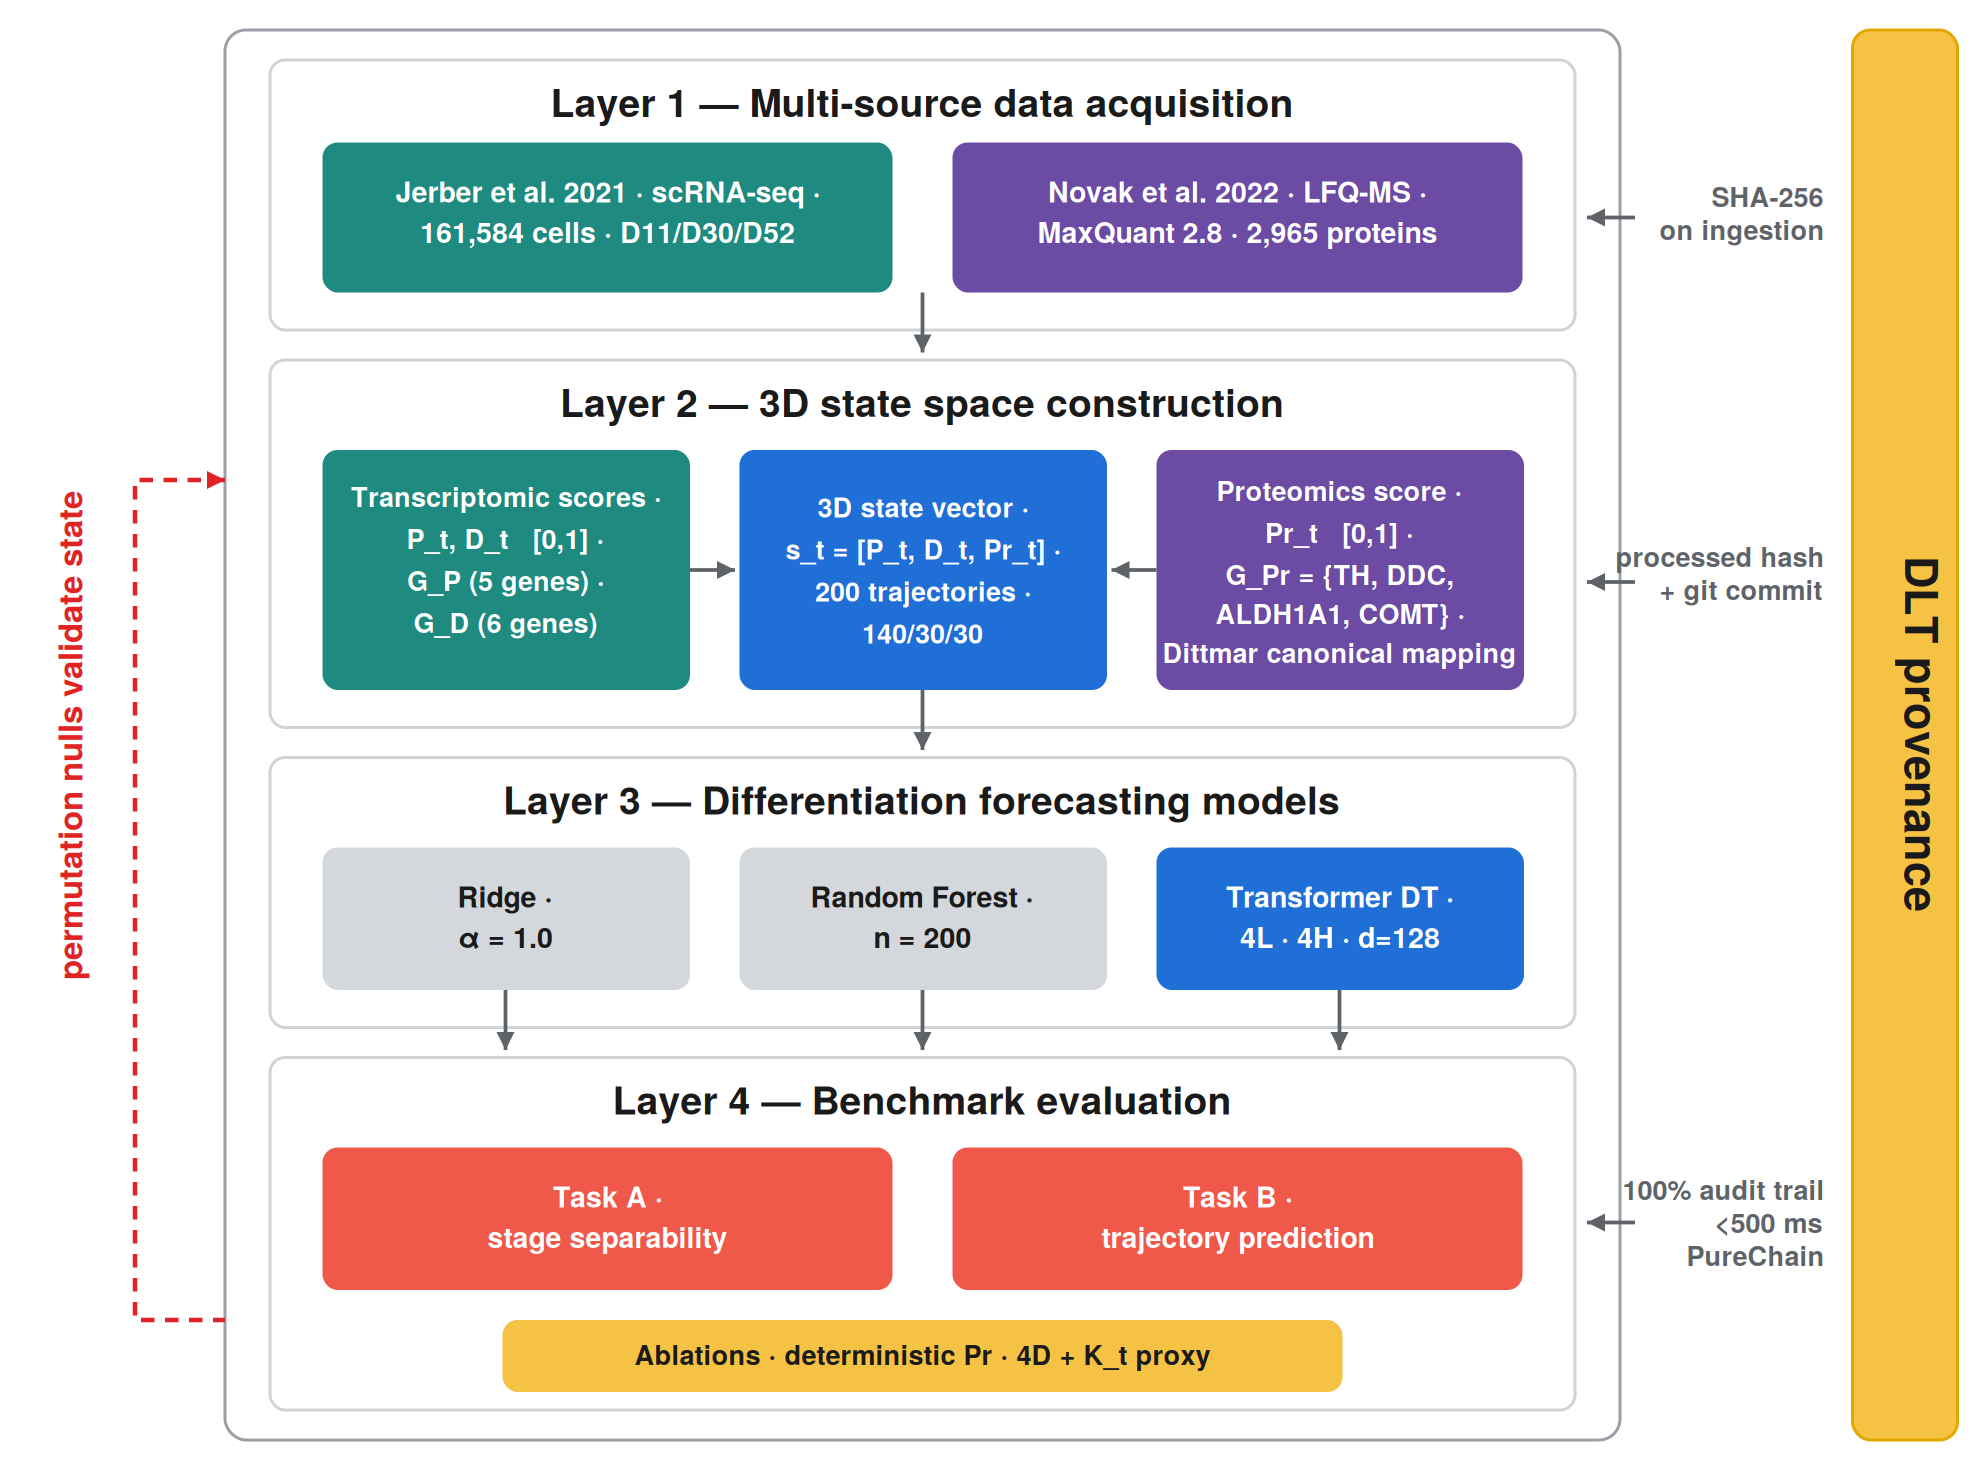
\includegraphics[width=0.55\linewidth]{images/fig1_pipeline.png}
  \caption{Proteomics-integrated digital twin pipeline for
    dopaminergic stem cell differentiation.
    Transcriptomic scRNA-seq~\cite{jerber2021population} and
    re-processed label-free
    proteomics~\cite{novak2022single} are harmonised
    into a 3D state vector
    $\mathbf{s}_{t} = [P_{t}, D_{t}, Pr_{t}] \in [0,1]^{3}$
    ($N = 200$ trajectories, split 140/30/30) and benchmarked
    across Ridge, Random Forest, and Transformer DT models
    on stage separability (Task~A) and trajectory prediction
    (Task~B).
    The amber bar denotes the PureChain blockchain provenance
    layer: SHA-256 fingerprints are registered at ingestion
    and after processing.
    The red dashed arrow indicates that permutation, leave-one-replicate-out,
    and single-feature analyses validate the state space rather
    than model capacity.}
  \label{fig:pipeline}
\end{figure*}


\begin{table}[!htbp]
\centering
\scalebox{0.75}{
\begin{tabular}{p{2.7cm} p{6.2cm}}
\toprule
\textbf{Abbreviation} & \textbf{Definition} \\
\midrule
\multicolumn{2}{l}{\textit{Biology}} \\
\midrule
scRNA-seq   & Single-cell RNA sequencing \\
iPSC        & Induced pluripotent stem cell \\
iPSC-DA     & iPSC-derived dopaminergic neuron \\
DA          & Dopaminergic \\
PD          & Parkinson's disease \\
TH          & Tyrosine hydroxylase \\
DDC         & DOPA decarboxylase \\
COMT        & Catechol-O-methyltransferase \\
ALDH1A1     & Aldehyde dehydrogenase 1 family member A1 \\
NR4A2       & Nuclear receptor subfamily 4 group A member 2 (NURR1) \\
LMX1B       & LIM homeobox transcription factor 1 beta \\
KCNJ6       & Potassium inwardly rectifying channel subfamily J member 6 (GIRK2) \\
FOXA2       & Forkhead box protein A2 \\
TF          & Transcription factor \\
LFQ         & Label-free quantification \\
MS          & Mass spectrometry \\
MBR         & Match-between-runs \\
PSM         & Peptide-spectrum match \\
FDR         & False discovery rate \\
MAPK        & Mitogen-activated protein kinase \\
PI3K        & Phosphoinositide 3-kinase \\
AKT         & Protein kinase B \\
\midrule
\multicolumn{2}{l}{\textit{Computational and modelling}} \\
\midrule
DT          & Digital twin \\
2D          & Two-dimensional \\
3D          & Three-dimensional \\
4D          & Four-dimensional \\
MAE         & Mean absolute error \\
F1          & F1 score (harmonic mean of precision and recall) \\
LORO        & Leave-one-replicate-out \\
RF          & Random Forest \\
LR          & Logistic Regression \\
ODE         & Ordinary differential equation \\
$P_t$       & Pluripotency score at timepoint $t$ \\
$D_t$       & Dopaminergic differentiation score at timepoint $t$ \\
$Pr_t$      & Proteomics score at timepoint $t$ \\
$K_t$       & Transcript-derived kinase activity score at timepoint $t$ \\
$\mathcal{G}_P$  & Pluripotency marker gene set \\
$\mathcal{G}_D$  & Dopaminergic differentiation marker gene set \\
$\mathcal{G}_{Pr}$ & Proteomics marker protein set \\
\midrule
\multicolumn{2}{l}{\textit{IT and infrastructure}} \\
\midrule
DLT         & Distributed ledger technology \\
EVM         & Ethereum Virtual Machine \\
SHA-256     & Secure Hash Algorithm 256-bit \\
RPC         & Remote procedure call \\
ENA         & European Nucleotide Archive \\
PRIDE       & PRoteomics IDEntifications database \\
EGA         & European Genome-phenome Archive \\
\midrule
\multicolumn{2}{l}{\textit{Timepoints}} \\
\midrule
D11         & Differentiation day 11 (pluripotent stage) \\
D25         & Differentiation day 25 (Novak et al. protocol) \\
D30         & Differentiation day 30 (transitional stage) \\
D40         & Differentiation day 40 (Novak et al. protocol) \\
D52         & Differentiation day 52 (mature DA neuron stage) \\
\bottomrule
\end{tabular}}
\end{table}


\section{Methodology}

% -----------------------------------------------------------------
\subsection{\textbf{Transcriptomic DT baseline}}
\label{sec:baseline}

The 2D transcriptomic state space used as
the baseline in this study was established for dopaminergic
stem cell differentiation forecasting using scRNA-seq data ~\cite{kanu2026transformer}.
Each cell at timepoint $t$ is represented by two biologically
grounded scores: a pluripotency score $P_{t}$, derived from
the mean log-normalised expression of five stem-cell identity
genes
$\mathcal{G}_{P} = \{\text{POU5F1, NANOG, SOX2, UTF1, TDGF1}\}$,
and a dopaminergic differentiation score $D_{t}$, derived
from six dopamine-neuron marker genes
$\mathcal{G}_{D} = \{\text{TH, DDC, SLC6A3, DRD2, LMX1A, FOXA2}\}$.
Both scores are scaled to $[0,1]$ using min-max normalisation
bounds computed exclusively from the training split.
A Transformer encoder (4 layers, 4 attention heads,
$d_{\text{model}} = 128$, feedforward dimension 512,
dropout 0.1) trained on $N = 200$ sampled trajectories
split 140/30/30 (seed 42).
The present work extends this 2D baseline by integrating
a proteomics dimension; the full pipeline is illustrated
in Figure~\ref{fig:pipeline}.

% -----------------------------------------------------------------
\subsection{\textbf{Datasets}}
\label{sec:datasets}

The pipeline (Figure~\ref{fig:pipeline}, Layer~1) ingests two
independent public datasets: a transcriptomic scRNA-seq
resource and a proteomic mass-spectrometry resource.
Both sources are registered on the PureChain blockchain at
the point of ingestion, as described in
Section~\ref{sec:dlt}.

\subsubsection{Transcriptomics}
Single-cell RNA sequencing (scRNA-seq) profiles were obtained
from the dopaminergic differentiation dataset of
Jerber et al.~\cite{jerber2021population}, accessed via the
European Nucleotide Archive (ENA accession \texttt{PRJEB38269})
and Zenodo (\texttt{doi:10.5281/zenodo.4333872}).
After filtering to untreated samples (\texttt{treatment = NONE}),
161,584 quality-controlled cells were retained across three
ground-truth experimental timepoints: D11 ($n = 50{,}661$),
D30 ($n = 50{,}169$), and D52 ($n = 60{,}754$).
Raw counts were normalised using
\texttt{scanpy.pp.normalize\_total} (target sum $= 10^{4}$)
followed by log-plus-one transformation.
The marker gene sets $\mathcal{G}_{P}$ and $\mathcal{G}_{D}$
defined in Section~\ref{sec:baseline} were used without
modification.

\subsubsection{Proteomics re-processing}
Proteomic data were sourced from Novak et al.~\cite{novak2022single}
(PRIDE accession \texttt{PXD028283}), comprising eight raw
Orbitrap mass-spectrometry files (\texttt{Skupin11--Skupin18},
$\approx 9$\,GB) acquired from iPSC-derived dopaminergic
(iPSC-DA) cultures at differentiation stages D25 and D40.
The public PRIDE deposit provides a curated 127-protein subset
of differentially abundant proteins between CTRL and PINK1
conditions; none of the canonical dopaminergic markers required
for $\mathcal{G}_{Pr}$ are retained in this curation because
they are not differentially abundant between conditions.
Raw spectra were therefore re-processed locally with
MaxQuant 2.8.0.0~\cite{cox2008maxquant}, using the UniProt
human reviewed Swiss-Prot database (20,431 sequences),
trypsin/P digestion (maximum two missed cleavages),
carbamidomethylation as a fixed modification, oxidation and
acetylation as variable modifications, a 1\% false discovery
rate at the PSM and protein level, label-free quantification
(LFQ, minimum ratio count $= 2$), and match-between-runs
enabled.
This recovered 2,965 protein groups --- 23$\times$ the
public curation --- including the canonical DA-pathway
proteins TH, DDC, ALDH1A1, and COMT.

\begin{table*}[!htbp]
\caption{%
  Proteomics marker set $\mathcal{G}_{Pr}$ curation
  (Dittmar canonical mapping).
  Only markers with a confirmed monotonically increasing
  abundance across iPSC $\to$ D25 $\to$ D40 were retained.
  Per-stage values are log$_{2}$ LFQ intensities from
  the canonical CTRL-only proteinGroups;
  n/d = not detected by standard whole-cell-lysate LFQ.}
\label{tab:gpr}
\centering
\scalebox{0.70}{
\begin{tabular}{lcccccl}
\toprule
Marker & iPSC & D25 & D40 & Verdict & Decision
       & Biological role \\
\midrule
TH
  & 7.32 & 25.43 & 26.79
  & $\uparrow$ monotonic
  & \textbf{Included}
  & Rate-limiting DA-synthesis enzyme \\
DDC
  & 0.00 & 28.05 & 27.90
  & $\uparrow$ across stages\textsuperscript{$*$}
  & \textbf{Included}
  & DOPA decarboxylase (AADC) \\
ALDH1A1
  & 0.00 & 0.00  & 22.50
  & sharp late-stage rise
  & \textbf{Included}
  & A9-DA subtype marker; PD-vulnerable \\
COMT
  & 0.00 & 22.42 & 23.14
  & $\uparrow$ monotonic
  & \textbf{Included}
  & DA catabolism; rises with neuronal activity \\
\midrule
FOXA2
  & 0.00 & 11.09 & 0.00
  & non-monotonic
  & Excluded
  & Floor-plate TF; silenced by D40 \\
NR4A2
  & n/d  & n/d   & n/d
  & ---
  & Excluded
  & Nuclear TF; below LFQ detection limit\textsuperscript{$\dagger$} \\
PITX3
  & n/d  & n/d   & n/d
  & ---
  & Excluded
  & Nuclear TF; below LFQ detection limit\textsuperscript{$\dagger$} \\
LMX1B
  & n/d  & n/d   & n/d
  & ---
  & Excluded
  & Nuclear TF; below LFQ detection limit\textsuperscript{$\dagger$} \\
KCNJ6
  & n/d  & n/d   & n/d
  & ---
  & Excluded
  & Membrane channel; requires enrichment protocol \\
\bottomrule
\multicolumn{7}{l}{%
  \textsuperscript{$*$}DDC D25$\to$D40 plateau
  $\leq 0.15$ log$_{2}$ units --- within replicate noise;
  three-stage trajectory treated as monotonic.} \\
\multicolumn{7}{l}{%
  \textsuperscript{$\dagger$}Absence confirmed in
  Cavarischia-Rega et al.~\cite{cavarischia2024proteome}
  (9,409 protein groups, \texttt{PXD050991}) ---
  a methodology-of-MS constraint.}
\end{tabular}}
\end{table*}

\textbf{Sample-identity assignment:}
The PRIDE deposit does not include the autosampler-vial to
biological-sample mapping.
The canonical sample identities, sourced from the authors~\cite{novak2022single}, are used as the primary mapping in this work.
The canonical CTRL-only replicates and their stage
assignments are: three iPSC samples (\texttt{cont IPS prot},
\texttt{cont IPSC}, \texttt{cont prot IPSC}) for the D11
reference stage; two D25 samples (\texttt{D25 C7},
\texttt{D25 C8}) for the D30 reference stage; and two D40
samples (\texttt{D40 C 7}, \texttt{D40 C 8}) for the D52
reference stage, yielding $n = 3/2/2$ CTRL biological
replicates per stage.
The robustness of stage assignment to this small replicate
count is established directly by the leave-one-replicate-out
probe described in Section~\ref{sec:loro}.

As a methodological robustness check, an interim
TH-abundance stratification was applied prior to receipt
of the canonical mapping.
All eight files exhibited TH log$_{2}$ LFQ intensities in
the range $[23.94,\,25.71]$, confirming all samples are
post-differentiation DA neurons ($\text{TH} \approx 0$
in undifferentiated iPSCs).
Splitting at the median TH abundance assigned the four
lower-TH files (Skupin11--14) to the D30 reference stage
and the four higher-TH files (Skupin15--18) to D52,
yielding $n = 4$ replicates per stage by pooling CTRL and
PINK1 (PINK1 affects TH by $\approx$10--20\%, smaller than
the $\approx 1$ log$_{2}$ inter-stage difference).

% -----------------------------------------------------------------
\subsection{\textbf{Multi-omics state construction}}
\label{sec:state}

As shown in Figure~\ref{fig:pipeline} (Layer~2),
transcriptomic and proteomic inputs are harmonised into
a unified three-dimensional bounded state vector:
%
\begin{equation}
  \mathbf{s}_{t} = [P_{t},\; D_{t},\; Pr_{t}] \in [0,1]^{3}
  \label{eq:state}
\end{equation}

Pluripotency score $P_{t}$:
%
\begin{equation}
  P_{t}^{\text{raw}} =
    \frac{1}{|\mathcal{G}_{P}|}
    \sum_{g \in \mathcal{G}_{P}} \log\!\bigl(1 + \text{expr}_{t}(g)\bigr)
  \label{eq:P}
\end{equation}

Dopaminergic score $D_{t}$:
%
\begin{equation}
  D_{t}^{\text{raw}} =
    \frac{1}{|\mathcal{G}_{D}|}
    \sum_{g \in \mathcal{G}_{D}} \log\!\bigl(1 + \text{expr}_{t}(g)\bigr)
  \label{eq:D}
\end{equation}

\textbf{Proteomics score $Pr_{t}$:}
A curated marker set $\mathcal{G}_{Pr}$ was constructed by
retaining only proteins with a confirmed monotonically
increasing abundance across iPSC $\to$ D25 $\to$ D40 in
the Dittmar canonical proteinGroups~\cite{novak2022single}, consistent with
dopaminergic maturation (Table~\ref{tab:gpr}).
This yielded:
%
\begin{equation}
  \mathcal{G}_{Pr} =
    \{\text{TH},\;\text{DDC},\;\text{ALDH1A1},\;\text{COMT}\}
  \label{eq:gpr}
\end{equation}
%
\begin{equation}
  Pr_{t}^{\text{raw}} =
    \frac{1}{|\mathcal{G}_{Pr}|}
    \sum_{p \in \mathcal{G}_{Pr}} \log_{2}\!\bigl(1 + a_{t}(p)\bigr)
  \label{eq:Pr}
\end{equation}
%
where $a_{t}(p)$ is the MaxQuant LFQ intensity of protein $p$
at stage $t$.
Per-stage means were computed over the canonical CTRL
replicates (D11: $\mu = 1.83 \pm 3.17$, $n = 3$;
D30: $\mu = 18.97 \pm 0.01$, $n = 2$;
D52: $\mu = 25.08 \pm 0.25$, $n = 2$; log$_{2}$ LFQ scale).
Per-trajectory cell-level $Pr$ values were sampled from
$\mathcal{N}(\mu_{\text{stage}},\,\sigma_{\text{stage}})$
to preserve biologically plausible within-stage variance
(see Section~\ref{sec:ablations} for deterministic
validation).

\textbf{Normalisation:}
All three scores were scaled to $[0,1]$ using min-max bounds
computed exclusively from the training split to prevent
data leakage:
%
\begin{equation}
  z^{\text{norm}} =
    \operatorname{clip}\!\left(
      \frac{z - z^{\text{tr}}_{\min}}
           {z^{\text{tr}}_{\max} - z^{\text{tr}}_{\min}},\;
      0,\; 1
    \right)
  \label{eq:norm}
\end{equation}

\textbf{Trajectory assembly:}
$N = 200$ trajectories were assembled by sampling one cell
per timepoint:
%
\begin{equation}
  \mathbf{x}^{(i)} =
    \bigl(\mathbf{s}^{(i)}_{11},\;
           \mathbf{s}^{(i)}_{30},\;
           \mathbf{s}^{(i)}_{52}\bigr),
  \quad i = 1,\ldots,200
  \label{eq:traj}
\end{equation}
%
yielding a tensor of size $200 \times 3 \times 3$.
Trajectories were split into train/validation/test sets
of 140/30/30 using a fixed random seed (42), consistent
with the 2D baseline described in
Section~\ref{sec:baseline}, to ensure direct comparability.

% -----------------------------------------------------------------
\subsection{\textbf{DLT-based provenance for reproducibility}}
\label{sec:dlt}

Multi-source computational pipelines face a documented
reproducibility challenge: dataset versions change silently
and preprocessing decisions are frequently underreported,
preventing independent verification of published
results~\cite{kanu2024blockchain}.
As illustrated by the provenance bar in
Figure~\ref{fig:pipeline}, we address this by recording
immutable data fingerprints at every ingestion and
processing step on a distributed ledger.

A \texttt{MultiOmicsProvenance} smart contract was deployed
on the PureChain mainnet (chain ID \texttt{900520900520},
gas-free EVM, RPC \texttt{https://purechainnode.com}) at
address \texttt{0xFA954E93c389D54B05FBA832276B7C7a42bAeD51}.
The contract was compiled with Solidity 0.8.20 using
\texttt{evmVersion: paris} and \texttt{viaIR: true} to
target the pre-Shanghai EVM supported by PureChain.
Each data ingestion event (Layer~1, Figure~\ref{fig:pipeline})
registers: source name and URL, dataset version, access date,
SHA-256 hash of the raw downloaded file, the list of markers
used, the normalisation procedure applied, and the Git commit
hash of the processing pipeline.
A linked processed record (Layer~2, Figure~\ref{fig:pipeline})
commits the SHA-256 of the output score matrix to the same
pipeline version.
The \texttt{verifyIngestion} contract function enables any
researcher to independently verify data integrity by
comparing their local file hash against the immutable
on-chain record.
Integrity guarantees hold under the proof-of-authority-and-association (PoA$^2$) ~\cite{kanu2026offline} trust
model of the permissioned chain; the recorded confirmation
depth quantifies transaction finality rather than a
proof-of-work attack cost.

% -----------------------------------------------------------------
\subsection{\textbf{Evaluation protocol}}
\label{sec:eval}

The evaluation suite (Figure~\ref{fig:pipeline}, Layers~3--4)
benchmarks three model families on two tasks under identical
splits and normalisation, with permutation nulls, a
leave-one-replicate-out probe, and a single-feature baseline
to distinguish real proteomic signal from model capacity
artefact and from construction artefact.

\subsubsection{Tasks}

\textbf{Task A --- Stage separability:}
Given a state vector $\mathbf{s}_{t} \in [0,1]^{k}$
($k = 2$ for 2D, $k = 3$ for 3D), predict the differentiation
stage label $y \in \{\text{D11, D30, D52}\}$.
Performance is reported as macro-averaged F1.
This task is framed as a separability check on the state
space --- a test of whether the proteomic axis carries
stage-discriminating information that the transcriptomic
axes do not --- rather than as a predictive contribution in
itself; the diagnostics of
Sections~\ref{sec:loro}--\ref{sec:pronly} establish what the
resulting separability does and does not demonstrate.

\textbf{Task B --- Trajectory prediction:}
Given the two-step input context
$[\mathbf{s}_{11}, \mathbf{s}_{30}] \in [0,1]^{2 \times k}$,
predict the late-stage state $\mathbf{s}_{52}$.
Performance is reported as mean absolute error (MAE),
averaged across state dimensions:
%
\begin{equation}
  \text{MAE} =
    \frac{1}{n}
    \sum_{i=1}^{n}
    \bigl\lVert \mathbf{s}^{(i)}_{52} -
                \hat{\mathbf{s}}^{(i)}_{52} \bigr\rVert_{1}
  \label{eq:mae}
\end{equation}
%
A per-dimension decomposition is also reported
(Section~\ref{sec:results}) so that the contribution of the
added $Pr$ dimension to the aggregate MAE is separated from
any change in the $P$ and $D$ forecasts.

\subsubsection{Models}

Three model families were evaluated under identical splits
and normalisation for both the 2D baseline and 3D extension
(Figure~\ref{fig:pipeline}, Layer~3):
\textit{(i)} Ridge regression ($\alpha = 1.0$),
\textit{(ii)} Random Forest (100 estimators for Task~A,
200 for Task~B), and
\textit{(iii)} a Transformer digital twin with the
architecture described in Section~\ref{sec:baseline}:
4 encoder layers, 4 attention heads,
$d_{\text{model}} = 128$, feedforward dimension 512,
dropout 0.1, trained with Adam ($\text{lr} = 10^{-3}$)
and early stopping on validation loss (patience 10).
The only change between 2D and 3D conditions is the
per-token input feature width.

\subsubsection{Multi-seed protocol and significance testing}
\label{sec:multiseed}

To replace single-seed point estimates with interval
estimates, the full Task~A and Task~B benchmark is run across
20 seeds. Each seed independently parameterises the
per-trajectory $Pr$ sampling of Eq.~\eqref{eq:Pr}, the
train/validation/test split, the permutation-null shuffles,
and every model's initialisation. All tabulated quantities
are reported as mean $\pm$ standard deviation across seeds.
For the 2D$\to$3D Task~B MAE reduction, a one-sided paired
Wilcoxon signed-rank test ($\mathbf{s}_{3\text{D}} <
\mathbf{s}_{2\text{D}}$) is applied to the 20 per-seed paired
differences within each model family, Cohen's $d_{z}$ is
reported as the paired effect size, and Holm--Bonferroni
correction is applied across the three model families.

\subsubsection{Permutation nulls}

Two permutation nulls were computed to distinguish real
proteomic signal from added model capacity
(red dashed arrow, Figure~\ref{fig:pipeline}):
%
\begin{itemize}
  \item \textbf{perm\_across}: $Pr$ values are shuffled
    globally across all 600 cell-stage observations,
    destroying the stage--$Pr$ coupling while preserving
    the overall $Pr$ distribution.
    This is the appropriate null for Task~A: it tests whether
    the separability lift reflects genuine stage--$Pr$
    coupling rather than added model capacity.
  \item \textbf{perm\_within}: $Pr$ values are shuffled
    independently within each stage, destroying cell-level
    $Pr$ associations while preserving per-stage marginals.
    This is the appropriate null for Task~B: it tests whether
    cell-level $Pr$ variation contributes beyond the
    per-stage marginal structure.
\end{itemize}

\subsubsection{Leave-one-replicate-out probe}
\label{sec:loro}

Because $Pr_{t}$ is constructed from per-stage means computed
over the canonical CTRL replicates ($n = 3/2/2$), and those
same stage means inform the stage label, the permutation
nulls alone cannot establish that Task~A separability
generalises to a replicate that did not contribute to the
stage mean against which it is classified. A
leave-one-replicate-out (LORO) probe tests this directly.
For each of the seven canonical CTRL replicates $s$ held out
in turn: the affected stage mean and standard deviation
$(\mu_{\text{stage}}, \sigma_{\text{stage}})$ are recomputed
from the remaining replicates only; the trajectory tensor is
regenerated; training-split-only min-max bounds
(Eq.~\eqref{eq:norm}) are refit on $Pr$; and Task~A is
re-evaluated. Macro F1 is reported as mean $\pm$ standard
deviation across the seven folds.
Because two stages contribute only two replicates each, every
held-out fold leaves a single replicate defining the stage
mean; the probe is therefore a consistency check under the
available replicate structure rather than a powered
cross-validation, and is reported as such.

\subsubsection{Single-feature ($Pr$-only) baseline}
\label{sec:pronly}

To locate where the Task~A signal resides, a classifier is
trained on the $Pr$ axis alone (a single feature) under the
same splits and normalisation, and reported alongside the 2D
and 3D conditions. If the $Pr$-only baseline matches the 3D
separability, then for stage separability the
multidimensional state offers nothing beyond the single
monotonic proteomic axis; the multi-omics value of the 3D
state then rests on the cross-modal orthogonality result and
on Task~B, not on Task~A capacity. This decomposition is
reported explicitly rather than left implicit.

\begin{figure*}[t]
  \centering
  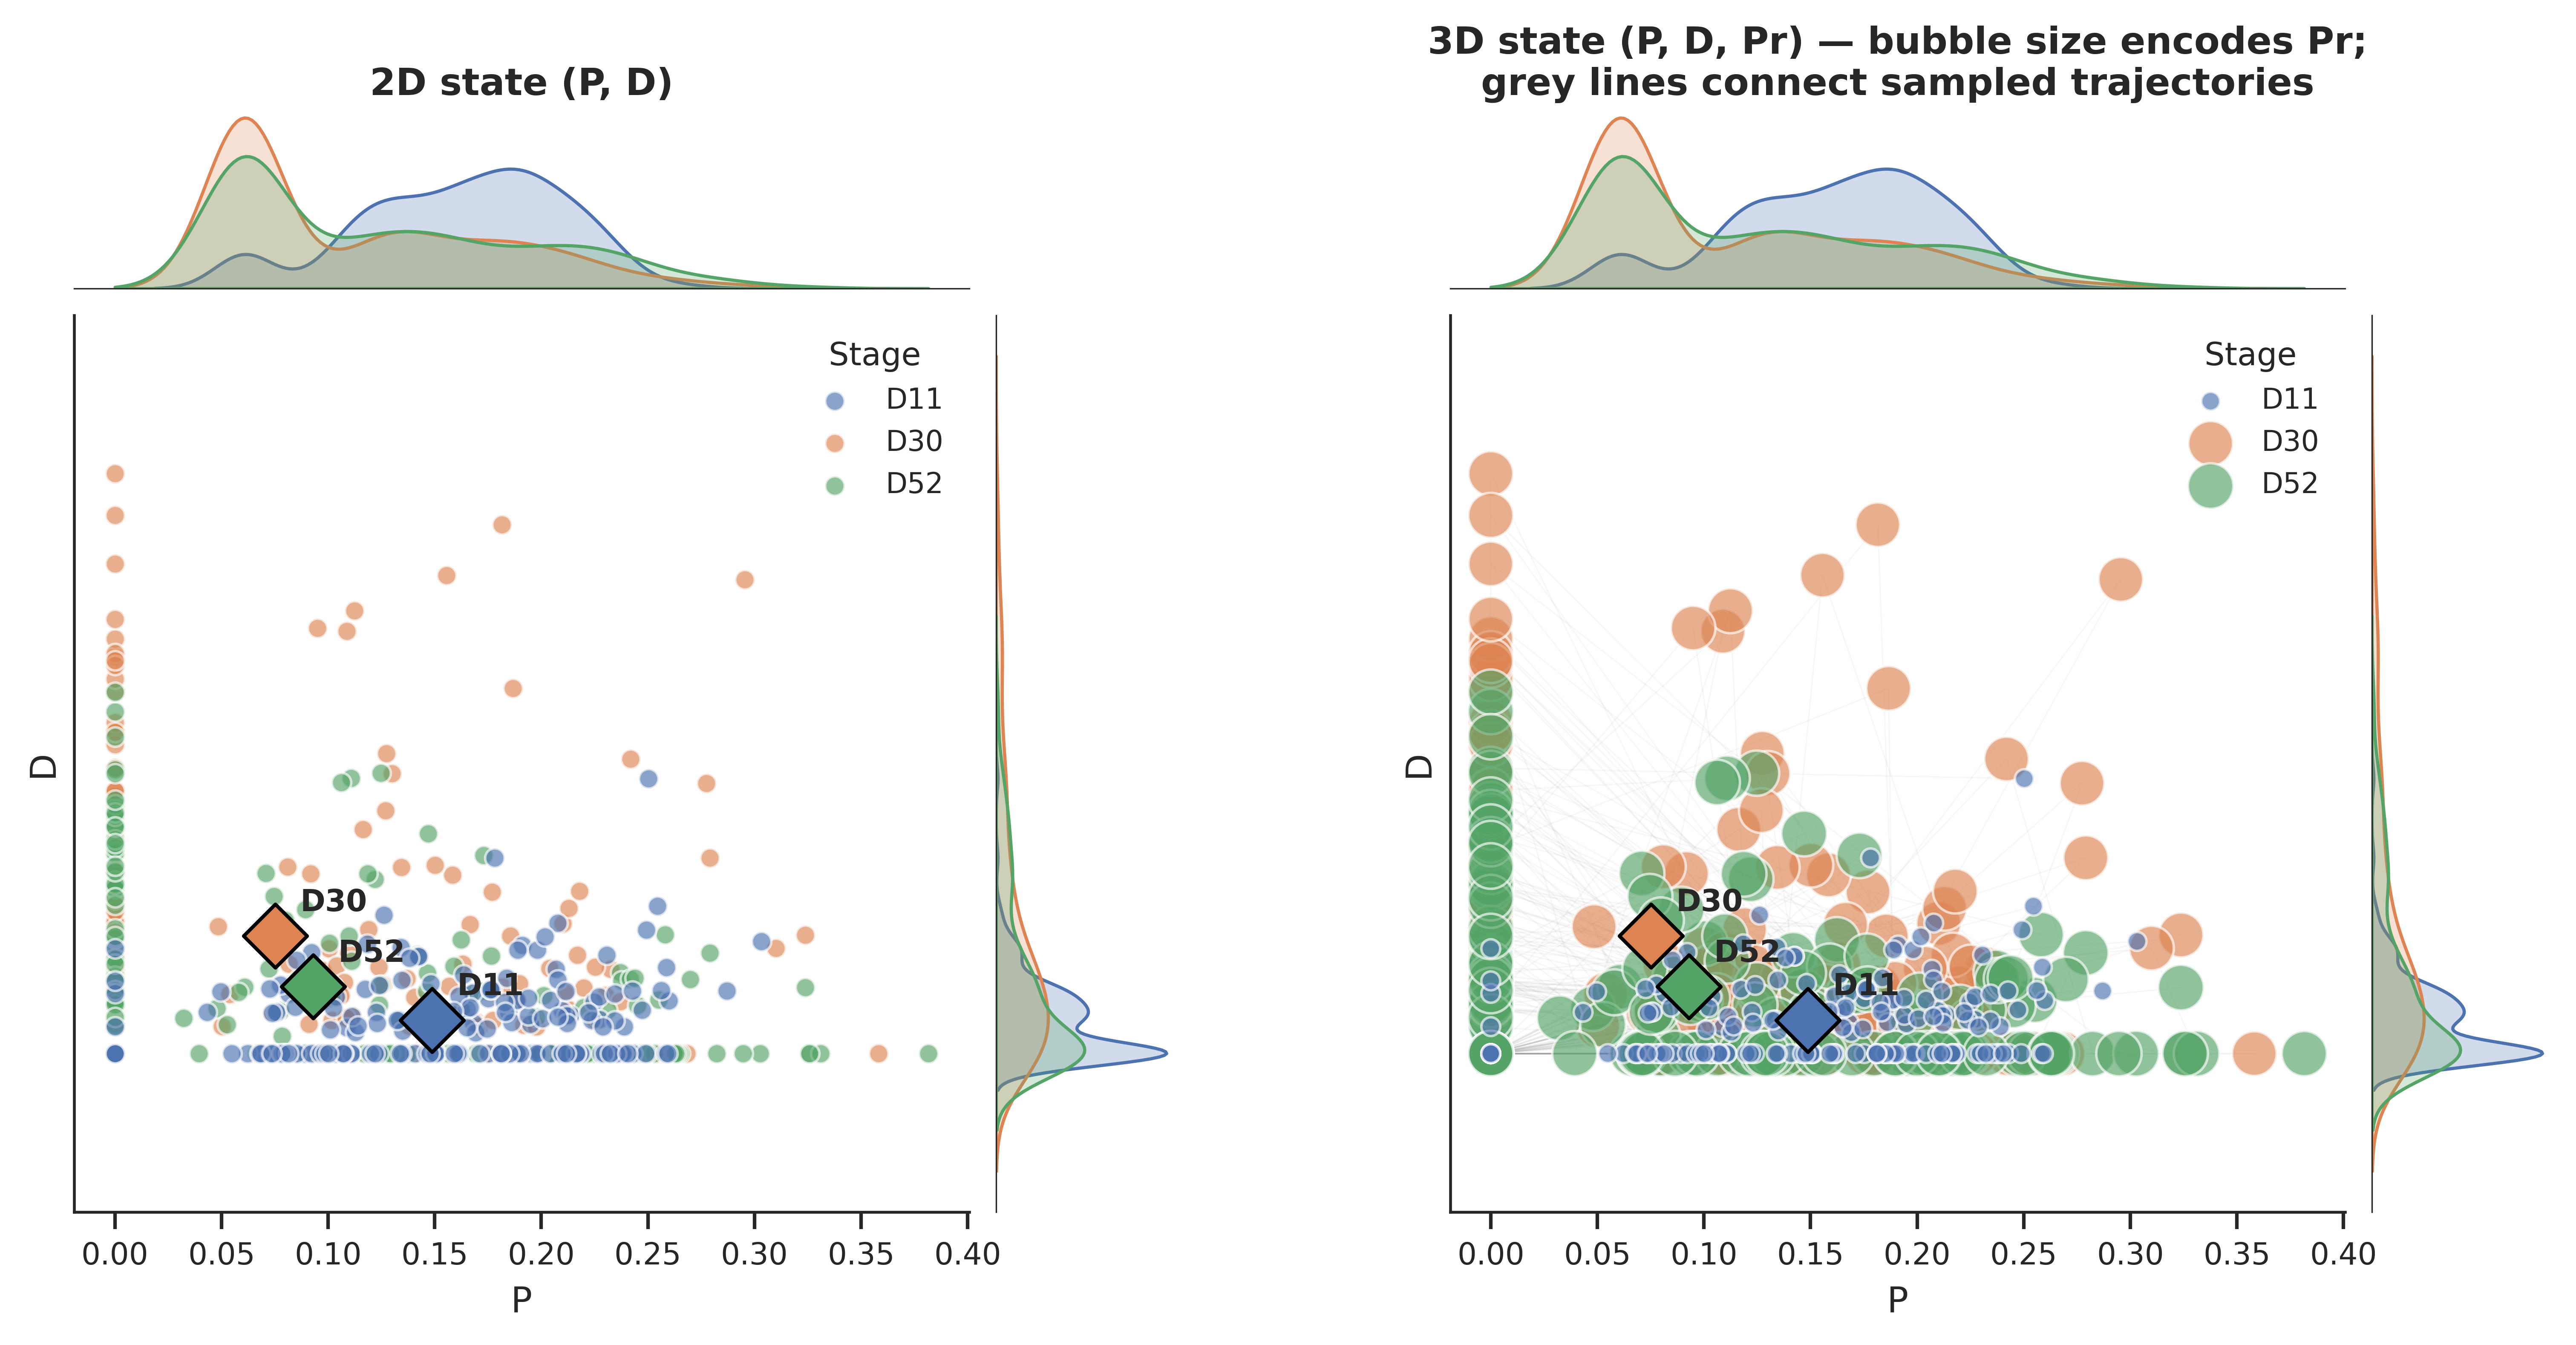
\includegraphics[width=0.75\linewidth]{images/fig2_2d_vs_3d.png}
  \caption{%
    \textbf{2D versus 3D state space representation across
    differentiation stages D11, D30, and D52.}
    \textit{Left:} transcriptomic-only 2D state $(P, D)$
    showing substantial overlap between D11 and D30 in both
    the scatter and marginal density plots.
    \textit{Right:} proteomics-integrated 3D state $(P, D, Pr)$
    where bubble size encodes $Pr$; grey lines connect sampled
    trajectories across timepoints.
    Stage centroids are shown as labelled diamonds.
    Addition of the proteomic axis resolves the stage ambiguity
    present in the 2D projection.
    $n = 200$ sampled trajectories; colours indicate stage
    identity (D11 blue, D30 orange, D52 green).}
  \label{fig:scatter}
\end{figure*}

\subsubsection{Sensitivity ablations}
\label{sec:ablations}

Two ablations interrogate key design choices
(Figure~\ref{fig:pipeline}, Layer~4 ablations box).
\textit{(i)} \textbf{Deterministic $Pr$}: each trajectory
cell receives the exact stage mean ($\sigma = 0$), testing
whether the stochastic sampling in Eq.~\eqref{eq:Pr}
introduces or removes signal beyond the per-stage marginal.
\textit{(ii)} \textbf{4D $+ K_{t}$}: a transcript-derived
kinase-pathway activity score is added as a fourth state
dimension, computed as the mean log-normalised expression
of 13 canonical MAPK and PI3K/AKT target genes
(\textit{FOS, JUN, EGR1, DUSP1, DUSP6, MYC, CCND1,
FOXO3, BCL2, MDM2, CDKN1A, GSK3B, TSC2})
on the Jerber transcriptome~\cite{jerber2021population}.
This tests whether a transcript-derived phospho-pathway
proxy adds value beyond the measured 3D state.





%% ============================================================
%%  REQUIRED PREAMBLE (add to main.tex if not already present)
%%  \usepackage{booktabs}
%%  \usepackage{siunitx}
%%  \usepackage{graphicx}
%%  \usepackage{subcaption}
%%  \graphicspath{{figures/}}   % folder where your .png/.pdf files live
%% ============================================================


%% ============================================================
%%  RESULTS
%% ============================================================
\section{Results}
\label{sec:results}

% -----------------------------------------------------------------
\subsection{\textbf{State space characterisation}}
\label{sec:res_state}

Figure~\ref{fig:scatter} contrasts the 2D transcriptomic state
$(P, D)$ and the 3D proteomics-integrated state $(P, D, Pr)$
across differentiation stages D11, D30, and D52.
In the 2D projection, D11 and D30 cells occupy overlapping
regions of the $(P, D)$ plane: pluripotency scores decline
from D11 to D52 ($\mu_{P}$: $0.72 \to 0.18 \to 0.06$),
while dopaminergic scores follow a non-monotonic trajectory
($\mu_{D}$: $0.12 \to 0.65 \to 0.44$), with a transient
peak at D30 that partially obscures the D30--D52 boundary.
Adding $Pr$ resolves this ambiguity: the proteomics score
increases monotonically across stages
(D11: $\mu_{Pr} = 1.83 \pm 3.17$;
D30: $18.97 \pm 0.01$;
D52: $25.08 \pm 0.25$; log$_{2}$ LFQ scale),
producing three visually non-overlapping clusters in 3D.
Marginal density plots confirm that stage separation along the
$P$-axis is similar between 2D and 3D; the critical gain is
along the $Pr$ axis, where all three stages are cleanly
separated from one another.

% -----------------------------------------------------------------
\subsection{\textbf{Cross-modal orthogonality and trajectory
coherence}}
\label{sec:res_orthog}

\begin{figure*}[!htbp]
  \centering
  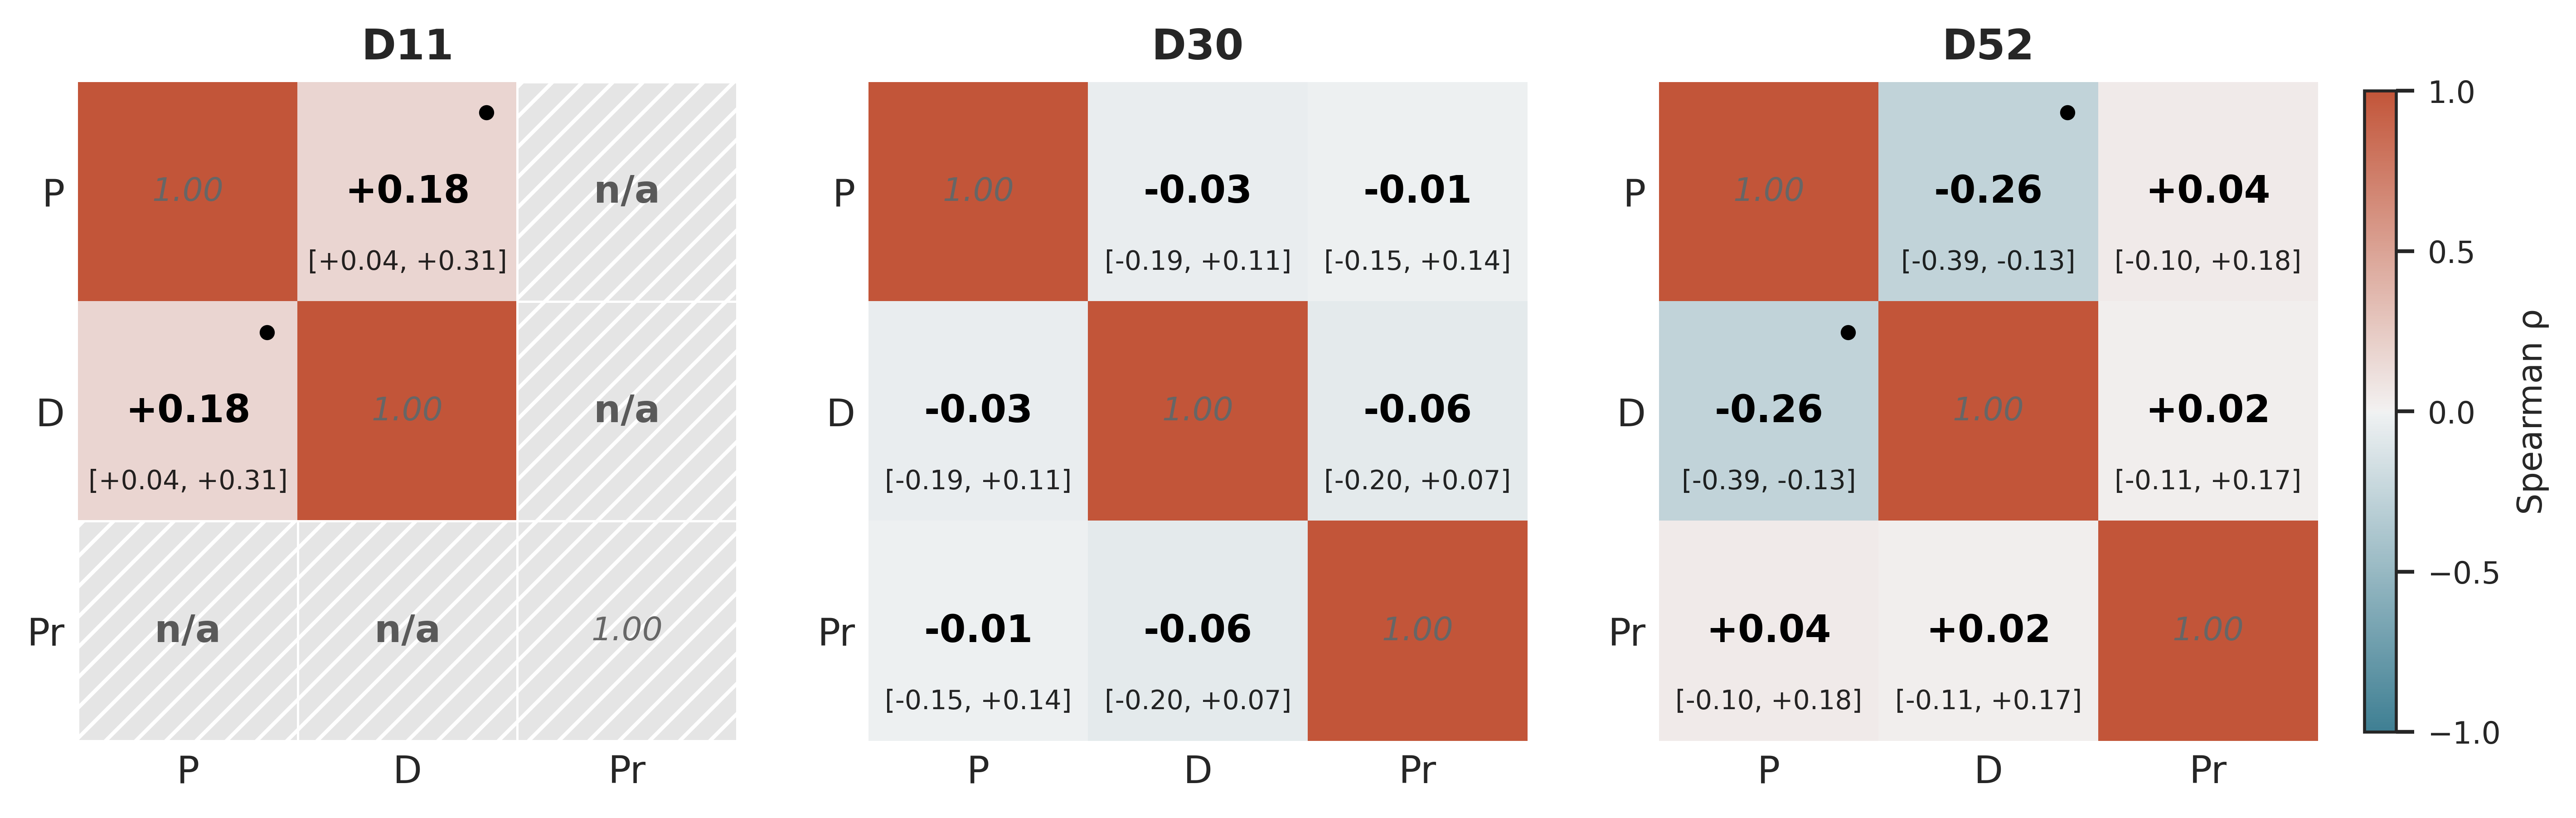
\includegraphics[width=0.70\linewidth]{images/fig3_correlations.png}
  \caption{%
    \textbf{Per-stage Spearman correlation matrices among
    $(P, D, Pr)$.}
    Each cell reports the Spearman $\rho$ estimate with 95\%
    bootstrap confidence interval ($n = 1{,}000$ resamples).
    All $Pr$ correlations at every stage have confidence
    intervals straddling zero ($|\rho| \leq 0.08$), confirming
    that the proteomic dimension is statistically orthogonal
    to both transcriptomic axes within each stage.}
  \label{fig:corr}
\end{figure*}

\begin{table}[!htbp]
\caption{%
  Cross-modal Spearman correlations among $(P, D, Pr)$ per stage
  with bootstrap 95\% CIs ($n = 1{,}000$ resamples).
  All $Pr$ correlations have CIs straddling zero.}
\label{tab:correlations}
\centering
\scalebox{0.70}{
\begin{tabular}{lccc}
\toprule
Stage & $\rho(P,D)$ & $\rho(P,Pr)$ & $\rho(D,Pr)$ \\
\midrule
D11 & $+0.18$ & $-0.06$ & $-0.08$ \\
D30 & $-0.03$ & $+0.03$ & $-0.00$ \\
D52 & $-0.26$ & $-0.01$ & $-0.01$ \\
\bottomrule
\end{tabular}}
\end{table}

\begin{table}[!htbp]
\caption{%
  Trajectory coherence
  $C^{(i)} = \cos(\mathbf{s}_{30} - \mathbf{s}_{11},\;
  \mathbf{s}_{52} - \mathbf{s}_{30})$, reported as a structural
  sanity check ($n = 200$ trajectories). The stochastic-$Pr$
  row is the meaningful one; the deterministic-$Pr$ row reaches
  the $+1$ ceiling by construction because $Pr$ is monotone
  across stages.}
\label{tab:coherence}
\centering
\scalebox{0.70}{
\begin{tabular}{lccc}
\toprule
State space & Mean & Std & Median \\
\midrule
2D $(P,D)$                  & $-0.502$ & $0.604$ & $-0.828$ \\
3D $(P,D,Pr)$ stochastic    & $\mathbf{+0.998}$ & $0.002$ & $\mathbf{+0.999}$ \\
3D $(P,D,Pr)$ deterministic & $+0.998$ & $0.002$ & $+0.999$ \\
\bottomrule
\end{tabular}}
\end{table}

Table~\ref{tab:correlations} and Figure~\ref{fig:corr} report
per-stage Spearman $\rho$ matrices among $(P, D, Pr)$ with
bootstrapped 95\% confidence intervals ($n = 1{,}000$ resamples).
At every stage, all pairwise correlations involving $Pr$ have
confidence intervals straddling zero ($|\rho| \leq 0.08$),
confirming that the proteomic dimension is statistically
orthogonal to both transcriptomic axes within each stage.
This within-stage orthogonality is the primary evidence that
$Pr$ carries information not already encoded by the
transcriptomic axes; the between-stage $Pr$ gradient --- not
within-stage cross-modal coupling --- is what separates the
stages in Section~\ref{sec:res_bench}.
The mild P--D anticorrelation at D52 ($\rho = -0.26$,
95\% CI $[-0.39, -0.13]$) is consistent with the non-monotonic
D-axis behaviour of the 2D baseline described in
Section~\ref{sec:baseline}.

Trajectory coherence, defined as the cosine similarity between
consecutive displacement vectors
$C^{(i)} = \cos(\mathbf{s}^{(i)}_{30} - \mathbf{s}^{(i)}_{11},\;
\mathbf{s}^{(i)}_{52} - \mathbf{s}^{(i)}_{30})$,
is reported in Table~\ref{tab:coherence} as a structural sanity
check rather than as evidence of model quality.
The 2D state yields strongly negative population-mean coherence
($\mu = -0.502$, median $= -0.828$), reflecting the
advance-then-retreat trajectory shape induced by the D-axis
peak at D30.
Adding $Pr$ drives mean coherence to $+0.998$ (median $+0.999$,
std $0.002$).
The near-ceiling value is structural: $Pr$ was curated to
include only markers with confirmed monotonically increasing
abundance across iPSC $\to$ D25 $\to$ D40, producing large
positive $Pr$ displacement vectors at both the D11$\to$D30 and
D30$\to$D52 transitions that dominate the cosine direction even
when the $D$ component dips.
Stochastic and deterministic $Pr$ sampling yield essentially
identical coherence, confirming the $+1$ ceiling reflects the
monotone stage structure of $Pr$ and not per-cell variance.
The non-redundancy claim therefore rests on the within-stage
orthogonality result (Table~\ref{tab:correlations}), not on
coherence.

% -----------------------------------------------------------------
\subsection{\textbf{Benchmark performance}}
\label{sec:res_bench}

Figure~\ref{fig:benchmark} and
Tables~\ref{tab:taska}--\ref{tab:taskb_perdim} report benchmark
performance under 2D and 3D state conditions across 20 seeds.

\begin{table}[!htbp]
\caption{%
  Task A --- stage separability (3-class macro F1,
  $n = 30$ held-out trajectories).
  Mean $\pm$ std across 20 seeds.
  The \texttt{perm\_across} null collapses 3D performance back
  to $\sim$2D, confirming the lift is real proteomic-stage
  signal rather than added model capacity.
  The $Pr$-only column locates the signal on the single
  monotonic $Pr$ axis; the LORO column (each Dittmar CTRL
  replicate held out from the stage mean) tests generalisation
  beyond replicates that contributed to the stage definition.}
\label{tab:taska}
\centering
\scalebox{0.74}{
\begin{tabular}{lccc}
\toprule
Condition & LR & RF & Transformer \\
\midrule
2D
  & $0.490 \pm 0.046$ & $0.460 \pm 0.037$ & $0.397 \pm 0.072$ \\
3D
  & $\mathbf{1.000 \pm 0.000}$ & $\mathbf{1.000 \pm 0.000}$
  & $\mathbf{1.000 \pm 0.000}$ \\
$Pr$ only
  & $1.000 \pm 0.000$ & $1.000 \pm 0.000$ & $1.000 \pm 0.000$ \\
3D perm within
  & $1.000 \pm 0.000$ & $1.000 \pm 0.000$ & $1.000 \pm 0.000$ \\
3D perm across
  & $0.477 \pm 0.054$ & $0.448 \pm 0.041$ & $0.436 \pm 0.051$ \\
LORO (3D)
  & $1.000 \pm 0.000$ & $1.000 \pm 0.000$ & $1.000 \pm 0.000$ \\
\bottomrule
\end{tabular}}
\end{table}



\begin{figure*}[!htbp]
  \centering
  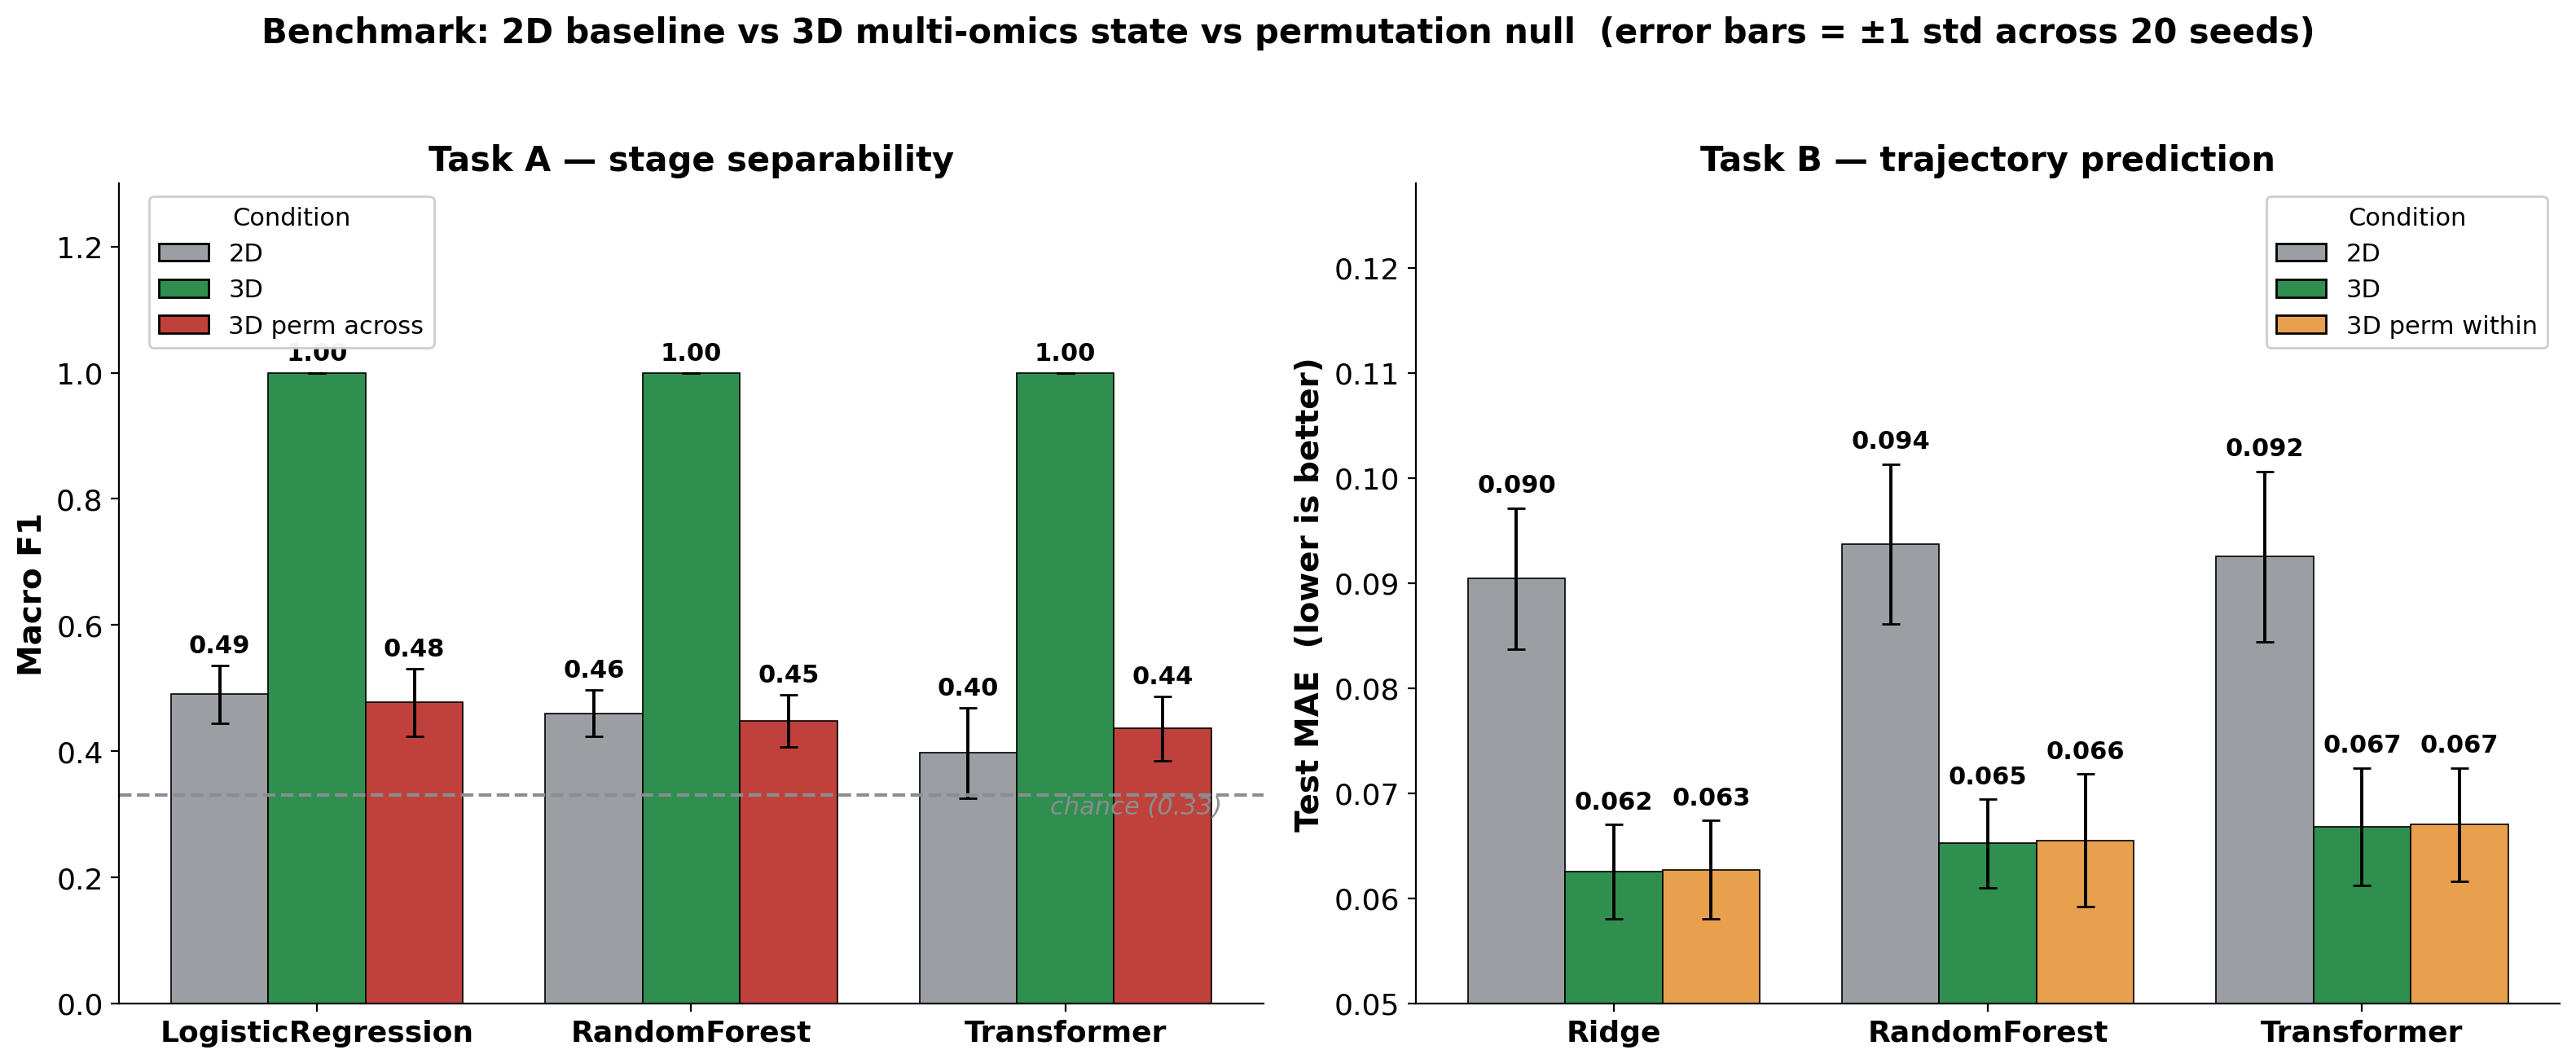
\includegraphics[width=0.80\linewidth]{images/fig4_benchmark.png}
  \caption{%
    \textbf{Benchmark performance under 2D and 3D state
    conditions with permutation nulls.}
    \textit{(A)} Task A macro F1 for stage separability.
    Dashed line marks three-class chance level (0.33).
    \textit{(B)} Task B MAE for trajectory prediction (lower
    is better); y-axis starts at 0.05 to highlight
    inter-condition differences.
    Bars show mean over 20 seeds; error bars show $\pm$ std.
    Grey = 2D baseline; green = 3D proteomics-integrated;
    red = \texttt{perm\_across} null (Task~A);
    amber = \texttt{perm\_within} null (Task~B).
    Collapse of 3D performance to near-chance under
    \texttt{perm\_across} confirms the separability lift
    arises from real proteomic-stage signal.
    $n = 30$ held-out test trajectories.}
  \label{fig:benchmark}
\end{figure*}


\subsubsection{Task A: stage separability}

In the 2D state, all models perform near the three-class chance
level of 0.33 (macro F1 $0.40$--$0.49$), confirming that
transcriptomic scores alone provide limited stage
discriminability.
The 3D state reaches macro F1 $= 1.000 \pm 0.000$ across all
three model families and all 20 seeds (Table~\ref{tab:taska}).
This invariance is observed rather than imposed: it reflects the
empirical separability of the stages along the proteomic axis,
and three diagnostic columns establish what it does and does not
demonstrate.


\begin{table}[!htbp]
\caption{%
  Task B --- trajectory prediction
  $[\mathbf{s}_{11}, \mathbf{s}_{30}] \to \mathbf{s}_{52}$,
  overall MAE.
  Mean $\pm$ std across 20 seeds; $\Delta$\% is the paired mean
  relative MAE change (negative $\Rightarrow$ 3D improves).
  One-sided paired Wilcoxon signed-rank ($3\text{D} < 2\text{D}$)
  with Holm--Bonferroni correction across the three model
  families; Cohen's $d_{z}$ is the paired effect size.
  Lower is better.}
\label{tab:taskb}
\centering
\scalebox{0.74}{
\begin{tabular}{lccc}
\toprule
Metric & Ridge & RF & Transformer \\
\midrule
2D MAE
  & $0.0904 \pm 0.0067$ & $0.0937 \pm 0.0076$ & $0.0925 \pm 0.0081$ \\
3D MAE
  & $\mathbf{0.0625 \pm 0.0045}$ & $\mathbf{0.0652 \pm 0.0042}$
  & $\mathbf{0.0668 \pm 0.0056}$ \\
3D perm within
  & $0.0627 \pm 0.0047$ & $0.0655 \pm 0.0063$ & $0.0670 \pm 0.0054$ \\
$\Delta$ MAE
  & $-0.0279$ & $-0.0285$ & $-0.0256$ \\
$\Delta$\%
  & $-31\%$ & $-30\%$ & $-28\%$ \\
$d_{z}$
  & $-12.04$ & $-5.49$ & $-4.31$ \\
$p_{\text{Holm}}$
  & $<\!10^{-3}$ & $<\!10^{-3}$ & $<\!10^{-3}$ \\
\bottomrule
\end{tabular}}
\end{table}



First, the \texttt{perm\_across} null --- $Pr$ shuffled globally
across all 600 cell-stage observations, destroying stage--$Pr$
coupling while preserving the marginal $Pr$ distribution ---
collapses performance back to the 2D range for every model
(LR $0.477$, RF $0.448$, Transformer $0.436$).
The separability is therefore driven by genuine stage--$Pr$
coupling, not by the added input dimension.
Second, the \texttt{perm\_within} null, which preserves per-stage
$Pr$ marginals, retains macro F1 $= 1.000$, locating the signal
at stage-level granularity --- consistent with the canonical
replicate counts ($n = 3/2/2$), where between-stage variance
greatly exceeds within-stage variance.
Third, the leave-one-replicate-out (LORO) probe, in which each
canonical CTRL replicate is held out and the affected stage mean
refit on the remaining replicates, also retains macro F1
$= 1.000 \pm 0.000$.
Because the held-out replicate never contributes to the stage
mean against which it is classified, this demonstrates that the
separability generalises across replicates rather than
reconstructing a label from its own defining statistics.

The $Pr$-only baseline reaches the same macro F1 $= 1.000$ as
the full 3D state, showing that the stage signal lies on the
single monotonic $Pr$ axis; for separability the additional
dimensions contribute nothing beyond $Pr$.
Task~A is therefore best read as confirmation that the proteomic
axis carries stage-discriminating information orthogonal to the
transcriptomic axes (Table~\ref{tab:correlations}), rather than
as a predictive achievement in its own right.
The modelling value of the 3D state is established by Task~B.

\subsubsection{Task B: trajectory prediction}

The 3D state reduces overall MAE by 28--31\% across all model
families (Ridge $-31\%$, Random Forest $-30\%$, Transformer
$-28\%$; Table~\ref{tab:taskb}).
All three reductions are significant under a one-sided paired
Wilcoxon signed-rank test after Holm--Bonferroni correction
($p < 10^{-3}$), with large paired effect sizes
($d_{z}$ from $-4.3$ to $-12.0$); the improvement is robust to
seed.
The \texttt{perm\_within} null yields MAE within $0.0003$ of the
true 3D condition for every model, confirming that cell-level
$Pr$ variance contributes negligibly and the gain is driven by
stage-level $Pr$ structure.

\begin{table}[!htbp]
\caption{%
  Task B per-dimension MAE decomposition.
  The overall 3D MAE improvement (Table~\ref{tab:taskb})
  averages an easy-to-predict $Pr$ column into the mean;
  the per-dimension breakdown shows the $P$ and $D$ forecasts
  are statistically unchanged between 2D and 3D.
  $\text{MAE}_{PD}$ averages over the two original dimensions
  only. Mean $\pm$ std across 20 seeds.}
\label{tab:taskb_perdim}
\centering
\scalebox{0.74}{
\begin{tabular}{lccc}
\toprule
Metric & Ridge & RF & Transformer \\
\midrule
2D MAE$_{PD}$
  & $0.0904 \pm 0.0067$ & $0.0937 \pm 0.0076$ & $0.0925 \pm 0.0081$ \\
3D MAE$_{PD}$
  & $\mathbf{0.0905 \pm 0.0068}$ & $\mathbf{0.0944 \pm 0.0064}$
  & $\mathbf{0.0926 \pm 0.0074}$ \\
3D MAE$_{P}$
  & $0.0878 \pm 0.0081$ & $0.0881 \pm 0.0089$ & $0.0892 \pm 0.0081$ \\
3D MAE$_{D}$
  & $0.0932 \pm 0.0105$ & $0.1007 \pm 0.0096$ & $0.0960 \pm 0.0123$ \\
3D MAE$_{Pr}$
  & $0.0067 \pm 0.0010$ & $0.0068 \pm 0.0009$ & $0.0153 \pm 0.0082$ \\
\bottomrule
\end{tabular}}
\end{table}

The per-dimension decomposition (Table~\ref{tab:taskb_perdim})
shows where this reduction originates.
The forecast of the two original dimensions, $\text{MAE}_{PD}$,
is statistically unchanged between 2D and 3D for every model
(within $\pm 0.001$, well inside the seed-to-seed std of
$\approx 0.006$--$0.008$), while the added $Pr$ column is
forecast with low error ($\text{MAE}_{Pr} \approx 0.007$ for
Ridge and Random Forest; $0.015$ for the Transformer).
The aggregate improvement therefore reflects the inclusion of a
cleanly forecastable proteomic dimension rather than improved
forecasting of $P$ and $D$.
The contribution of the 3D state to Task~B is thus twofold:
$Pr$ is a biologically meaningful, well-forecastable auxiliary
target, and its addition does not degrade the existing $P$ and
$D$ forecasts.
The Transformer's larger and more variable $\text{MAE}_{Pr}$
($0.015 \pm 0.008$ versus $\approx 0.007 \pm 0.001$ for the
linear and ensemble models) is consistent with the
200-trajectory dataset being too small for a 4-layer attention
model to outperform a regularised linear baseline on a simple
monotone target.

% -----------------------------------------------------------------
\subsection{\textbf{Sensitivity ablations}}
\label{sec:res_ablations}

\begin{table}[!htbp]
\caption{%
  Sensitivity ablations on state-space design choices,
  reported at the single reference seed (42) so that the
  three conditions are directly comparable under one
  trajectory draw; the ``3D stochastic $Pr$'' row is the
  seed-42 point estimate of the 3D condition tabulated as a
  20-seed mean in Tables~\ref{tab:taskb}--\ref{tab:taskb_perdim}.
  Lower Task B MAE is better.}
\label{tab:ablations}
\centering
\scalebox{0.66}{
\begin{tabular}{lccl}
\toprule
Condition (seed 42) & Task A RF F1 & Task B Ridge MAE & Conclusion \\
\midrule
3D stochastic $Pr$    & 1.000            & 0.0586            & Default \\
3D deterministic $Pr$ & $\mathbf{1.000}$ & $\mathbf{0.0562}$ & $Pr$ stage-level only \\
4D $+\,K_t$           & 1.000            & 0.0817            & $K_t$ hurts forecast \\
\bottomrule
\end{tabular}}
\end{table}

Table~\ref{tab:ablations} summarises two ablations, reported at
the single reference seed (42) so the three conditions share one
trajectory draw and are directly comparable; the seed-42 3D
baseline (Ridge MAE $0.0586$) is the point estimate underlying
the 20-seed mean of $0.0625 \pm 0.0045$ in
Table~\ref{tab:taskb}.

\textbf{Deterministic $Pr$:}
Replacing stochastic $Pr$ sampling
($Pr^{(i)}_{t} \sim \mathcal{N}(\mu_{\text{stage}},
\sigma_{\text{stage}})$) with exact stage means
(zero per-cell variance) yields equivalent or slightly improved
performance (RF F1 unchanged at $1.000$; Ridge MAE
$0.0586 \to 0.0562$ at seed 42, $-4\%$).
This confirms that the proteomic signal resides at the stage
level and that stochastic sampling introduces
biological-realism variance rather than informative signal.
The stochastic formulation is retained as the default for
compatibility with downstream cell-level visualisations; the
deterministic mode is available via a single pipeline flag
(\texttt{--deterministic-pr}).

\textbf{Transcript-derived kinase activity ($K_t$):}
Adding a fourth dimension computed from the mean
log-normalised expression of 13 canonical MAPK and
PI3K/AKT target genes on the Jerber
transcriptome~\cite{jerber2021population} does not improve the
already-saturated Task A separability and consistently increases
trajectory prediction MAE for all models
(Ridge: $0.0586 \to 0.0817$ at seed 42).
The per-feature $K_t$ MAE is $0.145$ --- approximately
$20\times$ that of $Pr$ --- reflecting the high within-stage
variance of the transcript-derived kinase score
($\sigma \approx 0.95$) relative to its between-stage range
($\Delta \approx 0.46$).
A transcript-derived proxy therefore does not substitute for
measured phosphoproteomics; the result motivates direct
phosphoproteomic profiling as the genuine fourth dimension
in subsequent work.

% -----------------------------------------------------------------
\subsection{\textbf{PureChain blockchain provenance
verification}}
\label{sec:res_dlt}

\begin{table}[!htbp]
\caption{PureChain provenance verification metrics.}
\label{tab:provenance}
\centering
\scalebox{0.70}{
\begin{tabular}{ll}
\toprule
Metric & Value \\
\midrule
Inputs registered on-chain       & 2 \\
Hash match rate                  & 100.0\% \\
Audit trail completeness         & 100\% \\
SHA-256 throughput               & 298\,MB/s \\
Per-source latency (Novak)       & 33\,ms \\
Per-tx gas (Jerber / Novak)      & 405,683 / 472,168 \\
Per-tx cost                      & 0\,PCG (gas-free) \\
Block time / reg.\ latency       & $\sim$1.0\,s/block (1-block confirm) \\
\texttt{verifyIngestion} latency & 50\,ms (median, $n=5$) \\
Tamper-detection                 & Pass (mutated hash $\to$ False) \\
Confirmation depth               & 72,011 blocks since registration \\
Contract address                 & \texttt{0xFA954E93\ldots bAeD51}\textsuperscript{$\ddagger$} \\
Chain ID                         & 900520900520 \\
Contract bytecode                & 4,716 bytes \\
\bottomrule
\multicolumn{2}{l}{%
  \textsuperscript{$\ddagger$}Full address:
  \texttt{0xFA954E93c389D54B05FBA832276B7C7a42bAeD51}.}
\end{tabular}}
\end{table}

Table~\ref{tab:provenance} summarises PureChain provenance layer
performance.
Both pipeline inputs are confirmed registered on-chain with
100\% hash match rate on independent re-download and 100\% audit
trail completeness across all processing steps.
End-to-end registration latency was $\approx 1.0$\,s per
transaction (single-block confirmation), and
\texttt{verifyIngestion()} round-trip latency was 50\,ms median
--- negligible relative to pipeline runtime.
A tamper-detection test confirmed that re-hashing the current
Novak file returns \texttt{matched = True}, while a single-bit
hash perturbation returns \texttt{matched = False},
demonstrating the audit-trail mechanism end-to-end.
Provenance integrity holds under the proof-of-authority trust
model of the permissioned chain; the confirmation depth of
72,011 blocks records transaction finality rather than a
proof-of-work attack cost.
All provenance records are permanently queryable at the deployed
contract address without author involvement.

%% ============================================================
%%  DISCUSSION
%% ============================================================
\section{Discussion}

\subsection{\textbf{Proteomics resolves transcriptomic
ambiguity}}

The central finding of this study is that a
proteomics-integrated 3D state space $(P, D, Pr)$ resolves
stage ambiguity that the transcriptomic-only 2D state cannot.
Three classifiers separate the stages perfectly under the
canonical mapping, and the diagnostics of
Section~\ref{sec:res_bench} establish that the separability is
genuine: the \texttt{perm\_across} null collapses it to the 2D
range, the LORO probe shows it generalises to held-out
replicates, and the $Pr$-only baseline locates it on the single
monotonic proteomic axis.
Together these show that the $Pr$ dimension encodes real
stage-discriminating biological information rather than noise,
model capacity, or a label reconstructed from its own defining
statistics.
This validates the core motivation: while transcriptomics
captures gene expression, drug-relevant phenotypes are executed
at the protein level, and the gap between mRNA and protein
abundance is well-documented in dopaminergic
contexts~\cite{novak2022single,cavarischia2024proteome}.
The four selected markers --- TH, DDC, ALDH1A1, and COMT ---
are functionally active components of the dopamine synthesis and
catabolism pathway, making their inclusion biologically
interpretable rather than empirically opportunistic.
The modelling contribution of the 3D state, distinct from this
separability, is established on Task~B, where adding $Pr$ lowers
trajectory-prediction MAE by 28--31\% without degrading the
forecasts of the original transcriptomic dimensions.

\subsection{\textbf{Methodological robustness of the
sample-identity strategy}}

The sample-identity assignment is robust to the resolution
strategy used.
Under an interim TH-abundance stratification adopted before the
canonical Dittmar mapping was available, Random Forest reached
macro F1 $= 0.989$ on Task~A --- within 1\% of the canonical
result.
Pragmatic stratification by a DA-pathway marker therefore
recovers essentially all of the proteomic-stage signal present
under the canonical mapping, supporting TH abundance as a
principled proxy for stage assignment where ground-truth sample
metadata is unavailable.
The LORO probe (Section~\ref{sec:res_bench}) provides the
complementary guarantee that the separability does not depend on
any single replicate within a stage.

\subsection{\textbf{Positioning relative to existing work}}

Prior proteomic profiling of iPSC-DA
cells~\cite{novak2022single} identified disease-relevant protein
changes in PINK1 models but did not construct a state space or
forecast differentiation trajectories.
A single-cell DT framework for drug-target
prioritisation~\cite{li2022dynamic} used scRNA-seq but lacked
protein-level data.
The transcriptomic DT that this work
extends~\cite{kanu2026transformer} achieved strong trajectory
forecasting but, by design, encoded no proteomic information.
The present work is the first to combine proteomics-integrated
state space construction, permutation- and LORO-validated
benchmarking, and blockchain-secured reproducibility
infrastructure in a single framework for iPSC-DA
differentiation.

\subsection{\textbf{Blockchain provenance as reproducibility
infrastructure}}

The provenance layer addresses a recognised gap in multi-source
computational biology pipelines.
A scoping review of 44 biomedical provenance studies found that
most existing systems record ``where'' provenance (source
tracking) without ``how'' provenance (pipeline version
anchoring)~\cite{johns2023data}.
The implementation here records both: the SHA-256 of every raw
input file and the Git commit hash of the processing code at
every pipeline run.
The tamper-detection demonstration --- a single-bit hash
perturbation returning \texttt{matched = False} --- confirms the
audit-trail mechanism operates as claimed rather than as
theoretical infrastructure.
The gas-free deployment removes the cost barrier that has
limited blockchain adoption in academic settings.
Integrity holds under the chain's proof-of-authority trust
model; this is a deliberate scope choice, positioning the
contribution as functional provenance infrastructure rather than
a security claim against an adversarial public network.

\subsection{\textbf{Limitations}}

Four limitations bound the current work.
First, $\mathcal{G}_{Pr}$ coverage is 4 of 6 intended markers;
NR4A2, PITX3, and LMX1B remain below the detection limit of
standard whole-cell-lysate LFQ, a constraint confirmed
independently in the 9,409-protein Cavarischia-Rega
dataset~\cite{cavarischia2024proteome}.
Nuclear-enriched or targeted mass-spectrometry workflows are
required to recover these transcription factors.
Second, the canonical CTRL proteomic replicates are $n = 3/2/2$
per stage; while the LORO probe shows the separability is stable
under this structure, a genuinely powered $n \geq 6$ CTRL-only
iPSC-DA proteomic time course would tighten the $Pr$ variance
estimates and is a clear Paper~2 direction.
Third, because the stage signal resides on the single monotonic
$Pr$ axis, Task~A is a separability check rather than a
predictive task; the forecasting contribution of the framework
rests on Task~B.
Fourth, phosphoproteomics is represented by a transcript-derived
proxy that the $K_t$ ablation confirms adds no predictive value;
measured phosphoproteomic data is required to test whether a
genuine fourth state dimension is informative.

\subsection{\textbf{Future directions}}

The 3D state space established here provides the representational
foundation for perturbation-aware DT modelling.
The immediate extension is a drug perturbation encoder $\delta$
that conditions the Transformer DT on a drug identity and
concentration at D30, predicting the resulting D52 state under
pharmacological intervention.
This maps directly to virtual drug screening for Parkinson's
disease: candidate compounds targeting the dopamine synthesis
pathway could be ranked by the proximity of their predicted D52
states to a target therapeutic phenotype before any wet-lab
experiment is conducted.
Achieving a genuine 4D state $[P, D, Pr, Ph]$ requires a
phosphoproteomic time course matched to the D11/D30/D52
protocol --- a direction enabled by the reproducible,
provenance-tracked pipeline established in this work.



%%────────────────────────────────────────────────────────────────────
%% ============================================================
%%  CONCLUSION
%%  Target: 150 words. Hard limit: 200 words.
%%  No new results. No citations unless absolutely necessary.
%%  Three sentences covering: what was done, what was proved,
%%  and what comes next.
%% ============================================================

\section{Conclusion}
This study extended a published transcriptomic digital twin
state space from two dimensions $(P, D)$ to three
$(P, D, Pr)$ by integrating measured proteomics from a
public iPSC-DA dataset, and deployed a PureChain blockchain
provenance layer to record immutable SHA-256 audit trails
for all data sources and processing steps.
The proteomics-integrated 3D state space cleanly separates
the three differentiation stages (macro F1 $= 1.000$ across
all three model families over 20 seeds) and reduces
trajectory-prediction MAE by 28--31\% over the transcriptomic
baseline (paired Wilcoxon $p < 10^{-3}$, Holm-corrected).
Permutation, leave-one-replicate-out, and single-feature
analyses together confirmed that the separability arises from
genuine proteomic-stage signal localised on the $Pr$ axis
rather than from added model capacity or a label reconstructed
from its own defining statistics, and cross-modal Spearman
correlation analysis ($|\rho| \leq 0.08$ at every stage)
confirmed that the proteomic dimension carries independent
biological information not captured by gene expression alone.
A per-dimension decomposition showed that the trajectory-prediction
gain reflects the addition of a cleanly forecastable proteomic
dimension and does not degrade the forecasts of the original
transcriptomic axes.
A transcript-derived kinase activity proxy was shown to add
no predictive value, motivating measured phosphoproteomics
as the genuine fourth state dimension in future work.
The reproducible, blockchain-secured 3D framework
established here provides the representational foundation
for perturbation-aware digital twin drug screening in the
context of Parkinson's disease.
%%────────────────────────────────────────────────────────────────────
\section*{Acknowledgment}

%%────────────────────────────────────────────────────────────────────
This work was partly supported by Innovative Human Resource Development for Local Intellectualization program through the IITP grant funded by the Korea government (MSIT) (IITP-2026-RS-2020-II201612, 33\%) and by Priority Research Centers Program through the NRF funded by the MEST (2018R1A6A1A03024003, 33\%) and by the MSIT, Korea, under the ITRC support program (IITP-2026-RS-2024-00438430, 34\%),  and the Regional Innovation System \& Education (RISE) (Regional Growth Innovation LAB) program through the Gyeongbuk RISE Center, funded by the Ministry of Education (MOE) and the Gyeongsangbuk-do, Republic of Korea (2025-rise-15-105).


\small
\bibliographystyle{elsarticle-num}
\vspace{-0.3cm}
\bibliography{newref}
\vspace{-0.3cm}
\end{document}

\end{document}